\chapter{MODELOS MATEMÁTICOS Y SIMULACIÓN}

%Contadores y formato para numeracion de elementos
\renewcommand{\thefootnote}{\arabic{footnote}}
\renewcommand{\theequation}{\arabic{chapter}-\arabic{equation}}
\renewcommand{\thefigure}{\arabic{chapter}.\arabic{figure}}
\renewcommand{\figurename}{Figura}
\renewcommand{\tablename}{\textbf{Tabla}}
\renewcommand{\thetable}{\textbf{\arabic{chapter}-\arabic{table}}}
\stepcounter{definitionN}
\stepcounter{exampleN}
\stepcounter{tableN}
\stepcounter{footN}
\stepcounter{algorithmN}
\providecommand{\abs}[1]{\lvert#1\rvert}
\providecommand{\norm}[1]{\lVert#1\rVert}
%%%agregue el paquete caption
\newpage

\section{INTRODUCCIÓN}\label{sec:intro}
Los agentes que interactúan en un territorio son, por regla general, móviles. Muy pocos de ellos son estáticos.  Por ejemplo, las personas se mueven a través del territorio mientras que un hospital es estático. Por esa razón es fundamental implementar agentes artificiales con la capacidad de moverse debido a que el agente afectará las variables de estado dependiendo del lugar del territorio en el cual se encuentre. \\
De acuerdo con (Ortiz Triviño, 2012) hay básicamente dos tipos de modelos que se utilizan en la simulación de la movilidad de agentes: Los modelos basados en trazas y los modelos artificiales o sintéticos. Los primeros son simplemente itinerarios que el programador le asigna al agente de forma explícita en una tabla.   Dicha tabla tiene dos campos uno para la hora y el otro para el lugar que debe desplazarse a esa hora.  De esta manera, el agente disparará la ejecución del movimiento a la hora indicada e irá al lugar señalado.\\
En simulación de sistemas complejos es más frecuente, sin embargo, implentar la segunda clase  de modelos.  En ellos la dirección y el desplazamiento del agente será guiado por un modelo probabilístico (como suele ocurrir en agentes de alta complejidad, por ejemplo, el gerente de la compañía petrolera, el alcalde del municipio, etc.)
\section{MODELOS DE MOVILIDAD SINTÉTICOS\\ ESTÁNDAR}\label{sec:movilityModels}
Existen numerosos y bien conocidos modelos de movilidad originados principalmente en ramas de la ingeniería de telecomunicaciones empleados para modelar matemáticamente dispositivos en redes de computadores dinámicas estocásticas (Bagchi \& Korea, n.d.).  esos modelos han sido también adaptados para implementar movimiento artificial en agentes artificiales.  Los modelos más destacados se describen brevemente a continuación. 
\subsection{Random Walk Mobility Model}
Bajo este modelo, un Agente se mueve desde su ubicación actual a una nueva ubicación eligiendo al azar una nueva dirección y velocidad.  Una trayectoria típica del movimiento de agentes bajo este esquema se puede ver en la Figura \ref{fig:1-1}.  La nueva velocidad y dirección se eligen entre rangos predefinidos; cada uno de los movimientos se lleva a cabo ya sea en un intervalo de tiempo  $t$ constante o una distancia $d$  constante, después de lo cual se calcula una nueva dirección y velocidad. Cuando un Agente llega a un límite de simulación (por ejemplo, la frontera del territorio), "rebota" con un ángulo que está determinado por la dirección entrante y la inclinación de la “pared” con la que golpea.\\

\begin{figure}[H]
\centering
\captionsetup{justification=centering,margin=2cm}
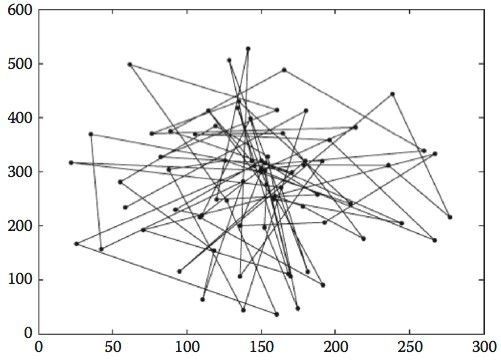
\includegraphics{chapters/chapter8/figures/1-1}
\caption{Trayectoria típica en el modelo Random Walk.}
\label{fig:1-1}
\end{figure}
Este modelo no tiene memoria, de ahí el nombre de caminata aleatoria. El patrón de movimiento de los Agentes en la simulación es, en consecuencia, un patrón al azar de itinerancia restringida a un pequeño segmento de la zona de simulación. 

\subsection{Random Waypoint}
Esta forma de movimiento incluye tiempos de pausa entre los cambios en la dirección y $/$ o velocidad. Un Agente móvil empieza inmóvil en un lugar por un período específico de tiempo.  A la expiración de este tiempo de duración, el Agente selecciona un destino al azar en el área de simulación y una velocidad que se distribuye uniformemente entre $[minSpd,m\acute{a}xSpd]$ . Después de alcanzar el destino tiene que esperar un tiempo de pausa especificada antes de repetir el proceso.

\subsection{Gauss-Markov}
El modelo de movilidad Gauss-Markov fue diseñado principalmente para adaptarse a diferentes niveles de aleatoriedad a través de un parámetro de ajuste. Inicialmente la velocidad y dirección actual se asignan a cada Agente móvil. Se fijan   intervalos de tiempo, el movimiento de cada Agente se produce mediante la actualización de la velocidad y dirección del Agente.  El valor de la velocidad y de la dirección en la instancia $n-\acute{e}sima$  se determina de acuerdo con las expresiones \ref{eqn:1-1} y \ref{eqn:1-2} en función de sus respectivos valores en la instancia $n-1$   de ahí el nombre de Markov y de dos variables aleatorias gaussianas.  Por esta razón, en la sección \ref{sec:gaussParamFam} se hace un estudio profundo de la familia de Gauss tanto en sus versiones univariada como multivariada. 

\begin{equation}
v_n=\alpha v_{n-1}+(1-\alpha)\ \mu_v+\sqrt{(1-\alpha^2) v_{x_{n-1}}}\ \ 
\label{eqn:1-1}
\end{equation}

\begin{equation}
d_n=\alpha d_{n-1}+(1-\alpha)\ \mu_d+\sqrt{(1-\alpha^2\ )\ d_{x_{n-1}\ }\ }\ \ 
\label{eqn:1-2}
\end{equation}

Empleando las expresiones \ref{eqn:1-1}  y \ref{eqn:1-2} se pueden calcular las coordenadas $(x,y)$  hacia donde el agente debe partir.  Para determinarlas se emplean las expresiones \ref{eqn:1-3} y \ref{eqn:1-4} .

\begin{equation}
x_n=x_{n-1}+v_{n-1}\ \ cos(\theta)\ d_{n-1}\ \ 
\label{eqn:1-3}
\end{equation}


\begin{equation}
y_n=y_{n-1}+v_{n-1}\ \ cos(\theta)\ d_{n-1} 
\label{eqn:1-4}
\end{equation}

Un hecho interesante que se desprende de las ecuaciones \ref{eqn:1-1} y \ref{eqn:1-2} , estudiado con el suficiente detalle matemático en (Ortiz Triviño, 2010), es que con $\alpha=0$  el movimiento resultante es de tipo Browniano.
En la evolución del sistema MIA se propone implementar otros modelos de movilidad en agentes lo que permitirá mayor flexibilidad y precisión en las simulaciones.  Para profundizar en ello puede verse también (Cao \& Das, 2012).


\section{FAMILIA PARAMÉTRICA DE GAUSS}\label{sec:gaussParamFam}
Se ha dicho antes que tanto la velocidad y la distancia en el modelo de movilidad seleccionado para los agentes del sistema MIA son variables aleatorias de Gauss.  Por esa razón, en esta sección se presenta formalmente esta familia.
\subsection{Familia de Gauss Uniparamétrica}
Cuando la variable aleatoria $X$   tiene una distribución normal con media $\mu_{X}$  y varianza $\sigma^{2}_X$ , se escribe  " $X$  es $N(\mu_{X},\sigma^{2}_X)$", o $X \sim N(\mu_{X},\sigma^{2}_X)$ . La función de densidad de  $X$ es entonces  la que se presenta en la expresión  \ref{eqn:1-5}.

\begin{equation}
f_X (x)=\frac{1}{{\sigma\sqrt{2\pi}}}e^{-\frac{1}{2} (x-\mu)^2/\sigma^2\ } para -\infty<x<\infty
\label{eqn:1-5}
\end{equation}
De acuerdo con (Mood, Graybill, \& Boes, 1974) se deduce que  $E(X)=\mu_X$  y  que $E(X-\mu)^{2}=\sigma^{2}_X$  . Es fácil, además, deducir que la función generadora de momentos de $X$ es $M_X(t)=e^{\mu t+\frac{1}{2}t^{2}\sigma^{2}}$. Esa deducción se realiza como sigue:\\
\begin{equation*}
M_X(t)=(\frac{1}{\sigma \sqrt{2\pi}})\int^{\infty}_{-\infty}exp[tx-\frac{1}{2}(x-\mu)^{2}/\sigma^{2}]dx 
\end{equation*}

\begin{equation*}
    =\frac{1}{\sigma \sqrt{2\pi}}\int^{\infty}_{-\infty}exp-\frac{1}{2}\{ [x-(\mu+t\sigma^{2})]^{2}-(2\mu t\sigma^{2}+t^{2}\sigma^{4})\}/\sigma^{2}dx
\end{equation*}
\begin{equation*}
    =e^{\mu t+\frac{1}{2}t^{2}\sigma^{2}}(\frac{1}{\sigma \sqrt{2\pi}})\int^{\infty}_{-\infty}exp[-(x-\mu-t\sigma^2)^2/2\sigma^2]dx
\end{equation*}
\begin{equation*}
    =e^{\mu t+\frac{1}{2}t^{2}\sigma^{2}}
\end{equation*}
Con este resultado es evidente que $\mu_X^{(1)}=\mu_X$, y que $\mu_X^{(2)}=\sigma_X^{2}+\mu_X^{2}$ , con lo cual $E(X-\mu_X)^2=\mu_X^{(2)}-\mu_X^2=\sigma_X^2$ .

\subsection{Distribución Normal Multivariada}
La extensión del caso univariado al multivariado de la familia de Gauss es importante por cuanto, por ejemplo, las coordenadas a las cuales se debe desplazar un agente tienen dos componentes y, para el modelo Gauss-Markov, ese comportamiento se modela con esta estructura probabilística. 
\subsubsection{Función de densidad}
Cuando las variables aleatorias en el vector  $X^\prime=[X_1,X_2,\cdots,X_n ]$  tiene una distribución normal multivariada con vector de medias  $\mu$ y matriz de la varianza-covarianza $V$ , se escribe "$X es N(\mu,V)"$    o  "$X\sim N(\mu,V)$ ". Cuando $E(X_i )=\mu$   para todo $i$ entonces $\mu=\mu_1$; y si los $X_i$   son mutuamente independientes, todos con la misma varianza $\sigma^2$ , entonces $V=\sigma^2\ I$   y se escribe  "$X$  es $N(\mu_1,\sigma^2 I)$". Esto es equivalente a la notación más usual  $ DNI(\mu,\sigma^2 )$ , pero manteniendo la notación de matriz de $N(\mu_1,\sigma^2 I)$ se da énfasis a que éste es simplemente un caso especial del caso general normal multivariado $N(\mu,V)$ .\\

El modelo supone que la matriz   $V$ es definida positiva. La función de densidad normal multivariada es la expresión \ref{eqn:1-6}. Nótese que en este contexto, el símbolo $^\prime$  en la expresión $(x-\mu)^\prime$, hace referencia a la transpuesta de $(x-\mu)^\prime$.
\begin{equation}
    f_X\ (x_1,x_2,\cdots,x_n\ )=\frac{e^{-\frac{1}{2}\ (x-\mu)^\prime\ V^{-1}\ (x-\mu)\ }}{(2\pi)^{\frac{1}{2} n}\ |V|^{\frac{1}{2}}\ }
    para  -\infty<X_i<\infty
\label{eqn:1-6}
\end{equation}
\subsubsection{Integral de Aitken}
Un resultado del cálculo integral que es particularmente aplicable a cualquier problema de la distribución normal multivariada es la integral de Aitken, presentada en la ecuación \ref{eqn:1-7} para  $A$ una matriz simétrica definida positiva de orden $n$ .  Con ella se puede verificar fácilmente que la expresión \ref{eqn:1-6} es, efectivamente, una estructura probabilística. 
\begin{equation}
    \int_{-\infty}^\infty...\int_{-\infty}^{\infty} e^{-\frac{1}{2} x^\prime Ax} dx_1...dx_n =(2\pi)^{\frac{1}{2}n} |A|^{-\frac{1}{2}}
    \label{eqn:1-7}
\end{equation}
Para establecer el resultado \ref{eqn:1-7}, nótese que debido a que  $A$ es definida positiva existe una matriz no-singular  $P$ tal que $P^\prime AP=I_n$  de tal forma que $|P^\prime AP|=|P|^2|A|=1$  y que $|P|=|A|^{-\frac{1}{2}}$ ; y sea  $x=Py$  con lo cual $x^\prime Ax=y^\prime P^\prime APy=y^\prime y$  por lo tanto:
 \begin{equation*}
     \int^{\infty}_{-\infty}...\int^{\infty}_{-\infty} e^{-\frac{1}{2}x^\prime Ax}dx_1...dx_n=\int^{\infty}_{-\infty}...\int^{\infty}_{-\infty} e^{-\frac{1}{2}y^\prime y}dy_1...dy_n/||P^{-1}||
 \end{equation*}
 
 \begin{equation*}
 \Box =||P||\int^{\infty}_{-\infty}...\int^{\infty}_{-\infty} exp(-\frac{1}{2}\sum^{n}_{i=1}y_i^{2})dy_1...dy_n    
 \end{equation*}
 
 \begin{equation*}
 \Box =||A||^{-\frac{1}{2}} \prod_{i=1}^{n}\{ \int^{\infty}_{-\infty}e^{-\frac{1}{2}y_i^{2}}dy_i\} 
 \end{equation*}
  \begin{equation*}
 \Box =(2\pi)^{\frac{1}{2}n}||A||^{-\frac{1}{2}}
 \end{equation*}
 La aplicación directa de la ecuación \ref{eqn:1-7} en la expresión \ref{eqn:1-6} muestra que:
 \begin{equation*}
     \int^{\infty}_{-\infty}...\int^{\infty}_{-\infty} f(x_1,x_2,...,x_n)dx_1...dx_n=(2\pi)^{\frac{1}{2}n}||V||^{-\frac{1}{2}}/(\sqrt{2\pi})^{n}||V||^{\frac{1}{2}}=1
 \end{equation*}
 como es de esperarse. 
\subsubsection{Función Generadora De Momentos}
En (Searle, 1971) se establece que, de una manera relativamente sencilla,  la función generadora de momentos para la distribución normal multivariada es  $M_X(t)=(2\pi)^{-\frac{1}{2}n}||V||^{-\frac{1}{2}}\int^{\infty}_{-\infty}...\int^{\infty}_{-\infty}exp[t^{\prime}x-\frac{1}{2}(x-\mu)^\prime V^{-1}(x-\mu)]dx_1...dx_n$de donde reformulando el exponente la expresión se convierte en : 
\begin{equation*}
    M_x(t)=(2\pi)^{-\frac{1}{2}n}||V||^{-\frac{1}{2}}\int^{\infty}_{-\infty}...\int^{\infty}_{-\infty}exp[-\frac{1}{2}(x-\mu-Vt)^{\prime}V^{-1}(x-\mu-Vt)+t^{\prime}\mu+\frac{1}{2}t^{\prime}Vt]dx_1...dx_n
\end{equation*}
\begin{equation*}
    \Box=\frac{e^{t^{\prime}\mu+\frac{1}{2}t^{\prime}Vt}}{(2\pi)^{\frac{1}{2}n}|V|^{\frac{1}{2}}}\int^{\infty}_{-\infty}...\int^{\infty}_{-\infty}exp[-\frac{1}{2}(x-\mu-Vt)^{\prime}V^{-1}(x-\mu-Vt)]dx_1...dx_n
\end{equation*}
Haciendo la transformación  $y=x-\mu-Vt$ de $x$  a $y$  para la cual el Jacobiano es la unidad, la integral se reduce entonces a la integral de Aitken con matriz $V^{-1}$ . Como consecuencia se llega a la expresión
\begin{equation}
    M_X(t)=\frac{e^{t^\prime\mu+\frac{1}{2}t^\prime Vt}(2\pi)^{\frac{1}{2}n}||V^{-1}||^{-\frac{1}{2}}}{(2\pi)^{\frac{1}{2}n}||V||^{\frac{1}{2}}}=e^{t^\prime\mu+\frac{1}{2}t^\prime Vt}
    \label{eqn:1-8}
\end{equation}
Diferenciando apropiadamente \ref{eqn:1-8} de la manera descrita en (Mood et al., 1974) se muestra que el vector de medias es   y la matriz de varianza-covarianza es $V$ .
\subsubsection{Distribuciones Marginales}
La definición de la distribución marginal de  $X_1,X_2,...,X_n$ a partir de los primeros $k$ $X$’s, es, de acuerdo con (Mood et al., 1974) la expresión \ref{eqn:1-9}.
\begin{equation}
    f_{X_1,...,X_k}(x_1,...,x_k)=\int^{\infty}_{\infty}...\int^{\infty}_{\infty}f(x_1,...,x_n)dx_{k+1}...dx_n
    \label{eqn:1-9}
\end{equation}
La función generadora de momentos de la  distribución \ref{eqn:1-9} es la expresión \ref{eqn:1-10}.
\begin{equation}
    M_{X_1,...,X_K}(t)=\int^{\infty}_{\infty}...\int^{\infty}_{\infty}e^{t_1x1+...+t_kx_k}f(x_1,...,x_n)dx_1...dx_k
    \label{eqn:1-10}
\end{equation}
Sustituyendo  $f(x_1,...,x_n)$  de acuerdo con la expresión \ref{eqn:1-6}, la ecuación \ref{eqn:1-10} se convierte en la ecuación \ref{eqn:1-11}.

\begin{equation}
\begin{split}
M_{X_1,...,X_K}(t) &=\int^{\infty}_{\infty}...\int^{\infty}_{\infty}e^{t_1x1+...+t_kx_k}f(x_1,...,x_n)dx_1...dx_k\\
&\Box=f.g.m \;de\; x_1,x_2,...,x_n, \;con\; t_{k+1}=...=t_n=0\\
&\Box=e^{t^{\prime}\mu+\frac{1}{2}t^{\prime}Vt},\;con\;t_{k+1}=...=t_n=0\\
\end{split}
\label{eqn:1-11}
\end{equation}
Para hacer las substituciones cuando $t_{k+1}=...=t_n=0$   se dividen o fraccionan $X$ , $\mu$ ,$V$   y $t$ , de esta forma $x_1^{\prime}=[x_1\;x_2...x_k]$    y $x_2^{\prime}=[x_{k+1}...x_n]$ con lo cual $x^{\prime}=[x_1^{\prime}\;x_2^{\prime}]$ ;  así,  conforme con este mismo procedimiento, $\mu^{\prime}=[\mu_1^\prime\;\mu_2^{\prime}]$   y $t^{\prime}=[t_1^\prime\;t_2^{\prime}]$  como también $\begin{bmatrix}
v_{11} & v_{12}\\
v_{21} & v_{22} 
\end{bmatrix} $ ; ahora, haciendo $t_2=0$  en \ref{eqn:1-11} se obtiene \ref{eqn:1-12}

\begin{equation}
M_{X_1,...,X_k}(t_1)=e^{t_1^{\prime}\mu_1+\frac{1}{2}t_1^{\prime}V_{11}t_1}
    \label{eqn:1-12}
\end{equation}

Por analogía con la expresión \ref{eqn:1-8} se tiene, por consiguiente, que la función de densidad marginal de   $X_1$ es  \ref{eqn:1-13}.
\begin{equation}
f_{X_1}(x_1,\cdots,x_k\ )=\frac{exp[-\frac{1}{2}\ (x_1-\mu_1\ )^\prime\ V_{11}^{-1}\ (x_1-\mu_1\ )]}{(2\pi)^{\frac{1}{2} k} |V_{11} |^{\frac{1}{2}} }
    \label{eqn:1-13}
\end{equation}
En comparación con \ref{eqn:1-6} es claro que $f_{X_1} (x_1,\cdots,x_k\ )$  es una distribución normal multivariada. Similarmente, también $f_{X_2 } (x_{k+1},\cdots,x_{n} )$  es \ref{eqn:1-14}.
\begin{equation}
f_{X_2}(x_{k+1},\cdots,x_n\ )=\frac{exp[-\frac{1}{2}\ (x_2-\mu_2)^\prime\ V_{22}^{-1}\ (x_2-\mu_2\ )]}{(2\pi)^{\frac{1}{2} (n-k)} |V_{22} |^{\frac{1}{2}} }
    \label{eqn:1-14}
\end{equation}
Así se concluye que las densidades marginales de la distribución normal multivariada son también normales multivariadas.  Nótese también que si  $V$ se toma como definida positiva igualmente lo serán  $V_{11}$ y$V_{22}$  . Además, con estas expresiones, su uso puede hacerse dividiendo  $V$ como en la expresión \ref{eqn:1-15}.
\begin{equation}
    V^{-1}=\begin{bmatrix}
V_{11} & V_{12}\\
V_{21} & V_{22} 
\end{bmatrix}^{-1}=\begin{bmatrix}
W_{11} & W_{12}\\
W_{21} & W_{22} 
\end{bmatrix}
\label{eqn:1-15}
\end{equation}
Con lo cual $V_{11}^{-1}=W_{11}-W_{12}\ W_{22}^{-1}\ W_{12}^\prime$   y  $V_{22}^{-1}=W_{22}-W_{12}^\prime\ W_{11}^{-1}\ W_{12}$.
\subsubsection{Distribuciones Condicionales}
Sea $f_X(x)$ la función de densidad conjunta de (todos) los $n$   valores de $X$  . Entonces la ecuación  \ref{eqn:1-16} da la distribución condicional de los primeros $k$ $X$'s dados los últimos $n-k$ $X$'s.
\begin{equation}
    f_{X_1|X_2} (\ x_1\ |\ x_2\ )=\frac{f_X\ (x_1,x_2,\cdots,x_n\ )}{f_{X_2\ }\ (x_{k+1},x_{k+2},\cdots,x_n\ )\ }
    \label{eqn:1-16}
\end{equation}
Sustituyendo las ecuaciones  \ref{eqn:1-6} y \ref{eqn:1-14} en \ref{eqn:1-16} se obtiene \ref{eqn:1-17}.
\begin{equation}
    f_{X_1\left|X_2\right.}\left(\left.x_1\right|x_2\right)=\frac{exp{\left\{-\frac{1}{2}\left[\left(x-\mu\right)^\prime V^{-1}\left(x-\mu\right)-\left(x_2-\mu_2\right)^\prime V_{22}^{-1}\left(x_2-\mu_2\right)\right]\right\}}}{\left(2\pi\right)^{\frac{1}{2}k}\left(\frac{\left|V\right|}{\left|V_{22}\right|}\right)^\frac{1}{2}}
    \label{eqn:1-17}
\end{equation}
Ahora, en términos de la partición de  $V$ y su inversa dada en \ref{eqn:1-15}, se tiene $\left(V_{11}-V_{12}V_{22}^{-1}V_{12}^\prime\right)^{-1} $  y  $V^{-1}=\left[\begin{matrix}W_{11}&-W_{11}V_{12}V_{22}^{-1}\\-V_{22}^{-1}V_{12}^\prime V_{11}&V_{22}^{-1}+V_{22}^{-1}V_{12}^\prime W_{11}V_{12}V_{22}^{-1}\\\end{matrix}\right]$ .  Por consiguiente el exponente en  \ref{eqn:1-17} se transforma en \\  $\left[\begin{matrix}\left(x_1-\mu_1\right)^\prime&\left(x_2-\mu_2\right)^\prime\\\end{matrix}\right]\left[\begin{matrix}W_{11}&-W_{11}V_{12}V_{22}^{-1}\\-V_{22}^{-1}V_{12}^\prime V_{11}&V_{22}^{-1}+V_{22}^{-1}V_{12}^\prime W_{11}V_{12}V_{22}^{-1}\\\end{matrix}\right]$ $\times\left[\begin{matrix}\left(x_1-\mu_1\right)\\\left(x_2-\mu_2\right)\\\end{matrix}\right]-\left(x_2-\mu_2\right)^\prime V_{22}^{-1}\left(x_2-\mu_2\right)$ lo que se simplifica a\\  $ =\left[\begin{matrix}\left(x_1-\mu_1\right)^\prime&\left(x_2-\mu_2\right)^\prime\\\end{matrix}\right]\left[\begin{matrix}I\\-V_{22}^{-1}V_{12}^\prime\\\end{matrix}\right]$ $W_{11}\left[\begin{matrix}I&-V_{12}V_{22}^{-1}\\\end{matrix}\right]\left[\begin{matrix}\left(x_1-\mu_1\right)\\\left(x_2-\mu_2\right)\\\end{matrix}\right]$ $=\left[\left(x_1-\mu_1\right)-V_{12}V_{22}^{-1}\left(x_2-\mu_2\right)\right]^\prime$ $W_{11}\left[\left(x_1-\mu_1\right)-V_{12}V_{22}^{-1}\left(x_2-\mu_2\right)\right]$.Además, usando el resultado para el determinante de una matriz dividida dado en (Searle, 1971) que se  resume en la expresión \ref{eqn:1-18} ,
\begin{equation}
    \left|V\right|=\left|V_{22}\right|\left|V_{11}-V_{12}V_{22}^{-1}V_{12}^\prime\right|=\left|V_{22}\right|\left|W_{11}^{-1}\right|
    \label{eqn:1-18}
\end{equation}
y teniendo presente \ref{eqn:1-19}
\begin{equation}
    \frac{\left|V\right|}{\left|V_{22}\right|}=\left|W_{11}^{-1}\right|
    \label{eqn:1-19}
\end{equation}
Es posible, luego de sustituir \ref{eqn:1-18} y \ref{eqn:1-19} en \ref{eqn:1-17}, obtener fácilmente \ref{eqn:1-20}
\begin{equation}
    f_{X_1|X_2}(x_1|x_2)=\frac{exp{\{-\frac{1}{2}[(x_1-\mu_1)-V_{12}V_{22}^{-1}(x_2-\mu_2)]^\prime W_{11}[(x_1-\mu_1)-V_{12}V_{22}^{-1}(x_2-\mu_2)]\}}}{(2\pi)^{\frac{1}{2}k}|W_{11}^{-1}|^\frac{1}{2}}
    \label{eqn:1-20}
\end{equation}
Demostrando, por simple comparación de la ecuación \ref{eqn:1-6} con la ecuación \ref{eqn:1-20} que la distribución condicional también es normal multivariada.   Este hecho se escribe formalmente en la ecuación \ref{eqn:1-21}.
\begin{equation}
    \left.X_1\right|X_2\sim N\left[\mu_1+V_{12}V_{22}^{-1}\left(x_2-\mu_2\right)W_{11}^{-1}\right]
    \label{eqn:1-21}
\end{equation}
\subsubsection{Independencia}
Supóngase que el vector $X'=\left[X_1,X_2,\cdots,X_n\right]$  se divide en  $p$ subvectores $X'=\left[X_1^\prime,X_2^\prime,\cdots,X_p^\prime\right]$  . Entonces una condición necesaria y suficiente (Searle, 1971) para que los vectores sean mutuamente independientes es, que en la partición correspondiente de $V=\left\{V_{ij}\right\}$  para $i,j=1,2,...,p$ , $V_{ij}=0$ , para $i\neq j.$ .  Prueba de esto se bosqueja a continuación. La f.g.m. de  $X$  está dada por la expresión \ref{eqn:1-8}, por lo tanto, se sigue la expresión \ref{eqn:1-22}.
\begin{equation}
    M_x\left(t\right)=e^{t^\prime\mu+\frac{1}{2}t^\prime V t}=exp{\left(\sum_{i=1}^{p}{t_i^\prime\mu_i}+\frac{1}{2}\sum_{i=1}^{p}\sum_{j=1}^{p}{t_i^\prime V_{ij}t_j}\right)}
    \label{eqn:1-22}
\end{equation}
Y si en la ecuación \ref{eqn:1-22},  $V_{ij}=0$  para $i\neq j$  esa expresión se reduce a
\begin{equation}
    M_X\left(t\right)=exp{\sum_{i=1}^{p}\left(t_i^\prime\mu_i+\frac{1}{2}t_i^\prime V_{ii}t_i\right)}=\prod_{i=1}^{p}exp{\left(t_i^\prime\mu_i+\frac{1}{2}t_i^\prime V_{ii}t_i\right)}
    \label{eqn:1-23}
\end{equation}
E invocando la propiedad demostrada en (Mood et al., 1974) según la cual la f.g.m. de la distribución conjunta de colecciones de variables independientes es el producto de sus f.g.m., se concluye que las $X_i$  son independientes. Recíprocamente, si esas  $p$ particiones son independientes, cada uno con su varianza-covarianza  $\gamma_{ii}$ se dice, entonces que la f.g.m. de la distribución conjunta es la expresión matemática dada en \ref{eqn:1-24}; donde $V=diag\left\{\gamma_{11},\gamma_{22},.\cdots\gamma_{pp}\right\}$  con $V_{ij}=0$  para $i\neq j$  .
\begin{equation}
    \prod_{i=1}^{p}exp{\left(t_i^\prime\mu_i+\frac{1}{2}t_i^\prime K_{ii}t_i\right)}=exp{\sum_{i=1}^{p}{\left(t_i^\prime\mu_i+\frac{1}{2}t_i^\prime K_{ii}t_i\right)=exp{\left(t^\prime\mu+\frac{1}{2}t^\prime V t\right)}}}
    \label{eqn:1-24}
\end{equation}
\section{MOVILIDAD GAUSS-MARKOV CON ATRACTORES}
Los agentes suelen moverse hacia puntos que los atraen debido a causas connaturales al sistema en el cual están inmersos. Por ejemplo, una comunidad humana puede tender a desplazarse hacia un área cercana a un nuevo pozo petrolero, o bien hacia el centro urbano más cerca, o hacia la rivera de un rio, entre tantos otros posibles factores de atracción. Este tipo de movimiento estocástico “normal” que tiene varios atractores puede simularse de una forma adecuada, véase (Ortiz Triviño, 2010),   empleando la familia de Gauss multivariada discutida en las secciones previas. \\
En la Figura \ref{fig:1-2} se presenta gráficamente esta situación. Supóngase que se ha determinado que en cierto territorio existen tres de estos atractores (puntos rojos en la figura), entonces las comunidades de agentes serán impulsadas a migrar hacia uno de estos puntos.  Ello significa que los agentes (o las comunidades de agentes) tienden a moverse de sus sitios actuales hacia algún lugar cercano. Para que el atractor no se convierta en una singularidad a la cual todos los agentes convergen (no sería lógico que la comunidad decida, por ejemplo, hacer su casa exactamente sobre el pozo petrolero) su distribución se rige con un comportamiento probabilístico basado en la familia de Gauss multivariada.  Muy en particular para el modelo implementado en el prototipo de software se ha tomado un   $n=2$ (dos dimensiones territoriales, es decir, un terreno plano, pero nótese que se pueden modelar muchas más dimensiones espacio-temporales).   Los círculos concéntricos de la Figura \ref{fig:1-2} representan las zonas a las cuales los agentes pueden llegar si se emplea el modelo gaussiano.
\begin{figure}[H]
\centering
\captionsetup{justification=centering,margin=2cm}
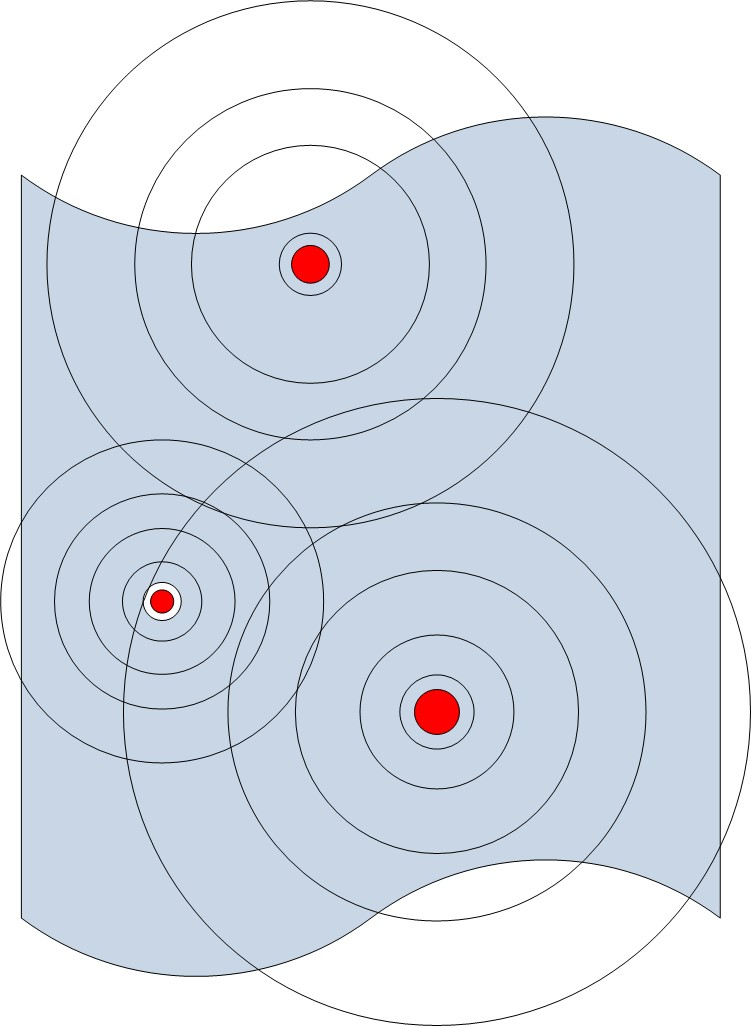
\includegraphics[scale=0.3]{chapters/chapter8/figures/1-2-1.jpg}
\caption{Un esquema con tres puntos de atracción.}
\label{fig:1-2}
\end{figure}
El objetivo es, entonces, que dado el agente  $A$, el cual se encuentra localizado en algún punto del territorio, determinar las nuevas coordenadas $(x_1,x_2)_A$  a las cuales debe desplazarse.  Para ello se emplea el método propuesto por (Ortiz Triviño, 2012) y que se resume como sigue: Cada atractor tendrá una fuerza (o ponderación) $p_k$  (usualmente se opta por $p_1$  como la fuerza que actúa sobre el agente y que lo obliga a no migrar o quedarse en el lugar en el cual se encuentra actualmente).  Naturalmente, de forma estándar,  $\sum_{k=1}^{n}p_k=1$ . Seguido, al tomar estas ponderaciones como una función de densidad de probabilidad, se genera un $k$  a partir de tales probabilidades. El  $k$ generado representará el atractor hacia el cual se verá forzado el agente a migrar. Ese lugar estará caracterizado por un punto a través del modelo gaussiano bidimensional con punto medio $\mu_X^{\left(k\right)}\in\mathbb{R}^2$  y una matriz de varianza-covarianza $V_k\in\mathbb{R}^2\times\mathbb{R}^2$  de donde se deben generar las coordenadas $\left(x_1,x_2\right)_A$ .  Para lograrlo es necesario contar con un generador de variables de Gauss univariadas y con ese método emplearlo para generar el punto en dos dimensiones, para mayores detalles matemáticos véase (Ortiz Triviño, 2012).
\subsection{Generador de una variable de Gauss Univariada}
En (Mood et al., 1974) se enuncia y demuestra que si $U_1\sim U\left(0,1\right)$  y $U_2\sim U\left(0,1\right)$ entonces $\sqrt{-2ln{\left(u_1\right)}}\times c o s{\left(2\pi u_2\right)}\sim N\left(0,1\right)$ .  A partir de este hecho, en (Ortiz Triviño, 2010) se propone  el Algoritmo \ref{alg:1-1}.  Aunque, de acuerdo con (Mood et al., 1974) existen métodos más eficientes para lograr este mismo resultado, dada su simplicidad resulta apto para esta aplicación.
\begin{algorithm} 
            \caption{Generador de una variable aleatoria normal estándar.}
            \label{alg:1-1}
            \begin{flushleft}
            \textbf{$\mathbb{R}:FUNCIONGeneradorNormalEstandar(u_1,u_2\in(0,1))$}\\
                \textbf{INICIO}\\
                \end{flushleft}
                \begin{algorithmic}
                \State$x\gets\sqrt{-2ln{(u_1)}}\times Cos(2\pi u_2);$    \\
                
                \textbf{RETORNAR($x$);}\\
                \end{algorithmic}
                
                
                \begin{flushleft}
                \textbf{FIN}\\
                \end{flushleft}
                
            
            
        \end{algorithm} 

\subsection{Generador de un vector dimensional de Gauss}
En (Ortiz Triviño, 2012) se presenta un algoritmo general para generar un vector de cualquier dimensión con estructura probabilística gaussiana dada en la expresión \ref{eqn:1-6}.  Ese algoritmo se ha adaptado para este documento en el caso particular cuando $n=2$ .  Esa adaptación corresponde al Algoritmo \ref{alg:1-3}.
\begin{algorithm}
    \caption{Generador de las coordenadas    para que migre un agente.}
    \label{alg:1-2}
    \textbf{$\mathbb{R}^2:FUNCIONMov\_GaussMarkov(P\in[0,1]^n,M\in{\mathbb{R}^2}^n,V\in{\mathbb{R}^2\times\mathbb{R}^2}^n;U\in(0,1)^4,u\in(0,1))$}
    \begin{flushleft}
    \textbf{INICIO}\\
    \end{flushleft}
    
    \begin{algorithmic}
    
    
    \State $k\gets SeleccionarNormal\left(P,u\right);$
    
    \State $[\begin{matrix}x_1\\x_2\\\end{matrix}]\gets GeneradorNormalBivariada(M[k],V[k],U)$
    \begin{flushleft}
    \textbf{Retornar$([\begin{matrix}x_1\\x_2\\\end{matrix}])$}
    \end{flushleft}
    
       
    \end{algorithmic}
    \begin{flushleft}
    \textbf{FIN}
    \end{flushleft}
\end{algorithm}


\begin{algorithm}
    \caption{Generador de una variable aleatoria normal estándar.}
    \label{alg:1-3}
    \textbf{$\mathbb{R}^2\;FUNCIONGeneradorNormalBivariada([\begin{matrix}\mu_1\\\mu_2\\\end{matrix}]\in\mathbb{R}^2,\Sigma=[\begin{matrix}\sigma_1^2&\sigma_{1,2}\\\sigma_{2,1}&\sigma_2^2\\\end{matrix}]\in\mathbb{R}^2\times\mathbb{R}^2;\{u_k\}_{k=1}^4\in(0,1)^4)$}
    \begin{flushleft}
    \textbf{INICIO}\\
    \end{flushleft}
    
    \begin{algorithmic}
    
    
    \State $\Sigma\gets CC^T;/*Descomposición\;de⬚\;holesky⬚*/$
    \State $z_1\gets GeneradorNormalEstandar\left(u_1,u_2\right);$
    \State $z_2\gets GeneradorNormalEstandar\left(u_3,u_4\right);$
    \State $x_1\gets\mu_1+c_{1,1}z_1;$
    \State $x_2\gets\mu_2+c_{1,1}z_1+c_{2,1}z_1+c_{2,2}z_2;$
    \begin{flushleft}
    \textbf{Retornar$(\left[\begin{matrix}x_1\\x_2\\\end{matrix}\right])$}
    \end{flushleft}
    
       
    \end{algorithmic}
    \begin{flushleft}
    \textbf{FIN}
    \end{flushleft}
\end{algorithm}




\subsection{Método de movilidad Gauss-Markov con múltiples atractores}
Al ejecutar el Algoritmo \ref{alg:1-4} se selecciona el $k-\acute{e}simo$  atractor hacia el cual se irá el agente al cual se le esté planeando un itinerario.
\begin{algorithm}
    \caption{: Generador del  $k-\acute{e}simo$ atractor.}
    \label{alg:1-4}
    \textbf{$\mathbb{N}:FuncionSelecionarNormal\left(P\in\mathbb{R}^n\right)$}
    \begin{flushleft}
    \textbf{INICIO}\\
    \end{flushleft}
    
    \begin{algorithmic}
    
    
    \State $u\gets Aleatorio\left(\right);$
    \State $i\gets1;$
    \State $F\gets p_1;$
    \begin{flushleft}
    MIENTRAS $(F\le u)$ HACER
    \end{flushleft}
    \begin{algorithmic}
     \State INICIO
     \State $\:\:\:i\gets i+1;$
     \State $\:\:\:F\gets F+p_i$
     \State FIN
    \end{algorithmic}
   
    \begin{flushleft}
    \textbf{Retornar$(i)$}
    \end{flushleft}
    
       
    \end{algorithmic}
    \begin{flushleft}
    \textbf{FIN}
    \end{flushleft}
\end{algorithm}
\\
Cada atractor está, como se mencionó anteriormente, caracterizado por un modelo basado en la distribución gaussiana; por eso, el Algoritmo \ref{alg:1-2} hace uso del Algoritmo \ref{alg:1-4} y del Algoritmo \ref{alg:1-3} para completar satisfactoriamente la tarea de encontrar las coordenadas  $(x_1,x_2)$ para determinado agente.\\
Para terminar, vale la pena indicar que al seleccionar  $n=2$ se asume un territorio plano.  El modelo, sin embargo, puede extenderse de tal manera que otras dimensiones tales como la social, puedan incorporarse en el concepto de movilidad de agentes (por ejemplo, posiblemente una comunidad indígena puede estar sesgada a migrar hacia pobladores de su misma raza).  Dicha generalización, no incluida aun en el prototipo, vale la pena incluirla en una nueva versión de la herramienta construida.


